\chapter{Bloed en de bloedsomloop}\label{ch:b2:blood-circulation}

In 1628 maakte William Harvey een rekensom. Het hart, schatte hij, bevat
ongeveer twee oncen \omterm{def:b2:blood-circulation:blood}{bloed} en klopt zeventig keer per minuut; zelfs als bij
elke slag maar een deel daarvan werd uitgestoten, zou het hart in een uur
meermaals het gewicht van het hele lichaam rondpompen. Het \omterm{def:b2:blood-circulation:blood}{bloed} kon niet in
dat tempo worden aangemaakt en verbruikt, zoals Galenus veertien eeuwen lang
had geleerd; het moest rond en rond gaan. Daarna toonde hij het aan: bind
een koord om de arm, en de \omterm{def:b2:blood-circulation:vessels}{aders} onder het koord zwellen op, niet erboven;
duw het \omterm{def:b2:blood-circulation:blood}{bloed} in een \omterm{def:b2:blood-circulation:vessels}{ader} naar de hand, voorbij een klep, en het gaat niet.
Het \omterm{def:b2:blood-circulation:blood}{bloed} wordt via de \omterm{def:b2:blood-circulation:vessels}{slagaders} uitgepompt, keert via de \omterm{def:b2:blood-circulation:vessels}{aders} terug, en
de hele vijf liter gaan elke minuut door het hart. Dit hoofdstuk gaat over
dat gesloten systeem --- wat \omterm{def:b2:blood-circulation:blood}{bloed} is, hoe het wordt geleid, de fysica van
zijn stroming door de vaten van de aorta tot een \omterm{def:b2:blood-circulation:vessels}{haarvat}, en de
uitwisseling in de \omterm{def:b2:blood-circulation:vessels}{haarvaten}, waar het allemaal om draait.

\section{Bloed}

\begin{definition}[De samenstelling van bloed]\label{def:b2:blood-circulation:blood}
\index{bloed}\index{plasma}\index{hematocriet}\index{rode bloedcel}\index{bloedplaatje}
Bloed is een weefsel in suspensie: ongeveer \qty{5}{L} bij een volwassene,
\qty{7}{\%} van de lichaamsmassa. Gecentrifugeerd scheidt het zich in
\emph{plasma} (\qty{55}{\%}: water, \qty{70}{g/L} eiwitten ---
albumine, globulinen, fibrinogeen --- en de zouten, suikers, lipiden,
gassen en hormonen die het vervoert) en cellen (\qty{45}{\%}, de
\emph{hematocriet}): \emph{rode bloedcellen} ($5\times 10^{12}$ per liter,
schijfjes van \qty{7}{\micro m} met twee holle kanten en zonder kern, elk
volgepakt met \num{280} miljoen hemoglobinemoleculen, met een levensduur
van 120 dagen en in het beenmerg gemaakt met twee miljoen per seconde),
\emph{witte bloedcellen} ($7\times 10^{9}$ per liter: neutrofielen,
lymfocyten, monocyten, eosinofielen, basofielen, de beweeglijke arm van de
immuniteit) en \emph{bloedplaatjes} ($3\times 10^{11}$ per liter,
fragmenten van beenmergcellen die wonden dichten en de stolling op gang
brengen). De rode bloedcellen vervoeren zuurstof --- \qty{200}{mL} per liter
bloed bij volledige verzadiging, zeventig keer wat water oplost --- en het
plasma vervoert al het andere, waaronder de \qty{20}{\%} van het
$\mathrm{CO_2}$ dat niet in de cellen zit, de warmte van de spieren naar
de huid, en de hormonen van \cref{ch:b2:cell-signalling} naar hun doelen.
Bloed is ook een oplossing onder \emph{\omterm{thm:b2:blood-circulation:oncotic}{oncotische druk}}: zijn eiwitten, die
de \omterm{def:b2:blood-circulation:vessels}{haarvaten} niet kunnen verlaten, oefenen een osmotische trek van
ongeveer \qty{25}{mmHg} uit, en die trek houdt het plasma in de
vaten.
\end{definition}

\begin{omfigure}
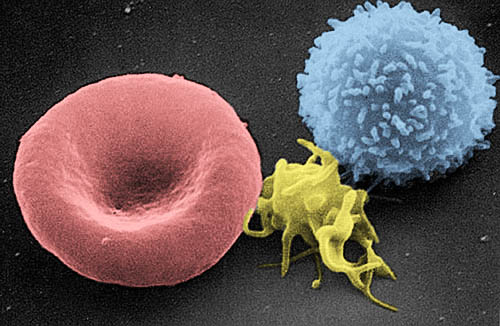
\includegraphics[width=0.5\linewidth]{images/book3/red-cells-nci.jpg}

{\small Een \omterm{def:b2:blood-circulation:blood}{rode bloedcel}, een \omterm{def:b2:blood-circulation:blood}{bloedplaatje} en een witte bloedcel (een
lymfocyt) onder de rasterelektronenmicroscoop: de drie cellulaire
bestanddelen van \omterm{def:b2:blood-circulation:blood}{bloed}, op dezelfde schaal getekend.}
\end{omfigure}

\begin{proposition}[Hemostase]\label{prop:b2:blood-circulation:clotting}
\index{hemostase}\index{stollingscascade}\index{fibrine}
Een doorgesneden vat wordt binnen enkele minuten in drie stappen gedicht.
Het vat trekt samen; \omterm{def:b2:blood-circulation:blood}{bloedplaatjes} kleven aan het blootgelegde collageen,
geven signalen af die meer \omterm{def:b2:blood-circulation:blood}{bloedplaatjes} rekruteren en activeren, en vormen
een prop; en een \emph{cascade} van plasmaproteasen, die elk de volgende
activeren (een twaalftal stollingsfactoren, de meeste in de lever gemaakt,
verscheidene afhankelijk van vitamine K), zet fibrinogeen om in onoplosbaar
\emph{fibrine}, waarvan de draden de prop tot een stolsel verweven. Een
cascade versterkt: een spoor van de trigger (weefselfactor uit de
beschadigde wand) eindigt in grammen fibrine. Ze moet ook worden ingeperkt:
antistollingsstoffen in het \omterm{def:b2:blood-circulation:blood}{plasma} (antitrombine, proteïne C) en op het
intacte endotheel beperken het stolsel tot de wond, en een tweede systeem,
de fibrinolyse, lost het op terwijl het vat geneest. Hemofilie is het
ontbreken van één factor; een trombose is een stolsel waar er geen gewenst
was, en de belangrijkste doodsoorzaak in rijke landen is een stolsel in een
kransslagader of een hersenslagader.
\end{proposition}

\section{Kringlopen}

\begin{definition}[Open en gesloten, enkelvoudig en dubbel]\label{def:b2:blood-circulation:circuits}
\index{open bloedsomloop}\index{gesloten bloedsomloop}\index{dubbele bloedsomloop}\index{kleine bloedsomloop}\index{grote bloedsomloop}
In een \emph{open} bloedsomloop (insecten, de meeste weekdieren) pompt een
hart \omterm{def:b2:blood-circulation:blood}{bloed} in een lichaamsholte, waar het de organen rechtstreeks omspoelt
en onder lage druk terugkeert; de stroming is traag en slecht gericht, en
de insecten hebben het gasprobleem van het \omterm{def:b2:blood-circulation:blood}{bloed} losgekoppeld door lucht
rechtstreeks naar de weefsels te leiden. In een \emph{gesloten} bloedsomloop
(ringwormen, inktvissen, gewervelden) blijft het \omterm{def:b2:blood-circulation:blood}{bloed} in vaten en wordt
het onder druk door \omterm{def:b2:blood-circulation:vessels}{haarvaten} gedreven, zodat de verdeling ervan orgaan
voor orgaan kan worden geregeld. Vissen hebben een \emph{enkelvoudige}
kringloop: hart
$\to$ kieuwen $\to$ lichaam $\to$ hart, zodat het \omterm{def:b2:blood-circulation:blood}{bloed} de weefsels bereikt
met de lage druk die na de \omterm{def:b2:blood-circulation:vessels}{haarvaten} van de kieuwen overblijft. Zoogdieren
en vogels hebben een \emph{dubbele} kringloop: het rechterhart drijft de
\emph{kleine bloedsomloop} aan (longen, lage druk, systolisch
\qty{25}{mmHg}) en het linkerhart, nadat het \omterm{def:b2:blood-circulation:blood}{bloed} is teruggekeerd, de
\emph{grote bloedsomloop} (lichaam, hoge druk, \qty{120}{mmHg});
de twee pompen staan in serie en verplaatsen dezelfde stroom, in rust
ongeveer \qty{5}{L} per minuut. Amfibieën en de meeste reptielen hebben een
hart met één ventrikel dat de twee stromen gedeeltelijk mengt --- het
tussenstadium. De dubbele kringloop maakt een warmbloedig metabolisme
mogelijk: hoge druk naar elk orgaan en een long die ertegen is beschermd.
\end{definition}
\begin{proof}[Bewijsmateriaal]
Harvey (1628) redeneerde vanuit de hoeveelheid --- het hierboven berekende
debiet --- en vanuit de bouw: de kleppen in de \omterm{def:b2:blood-circulation:vessels}{aders}, die Fabricius had
beschreven, laten alleen stroming naar het hart toe, zoals hij aantoonde door
op de \omterm{def:b2:blood-circulation:vessels}{aders} van een afgebonden arm te drukken; de kleppen van het hart laten
alleen stroming toe van atria naar ventrikels naar \omterm{def:b2:blood-circulation:vessels}{slagaders}; en \omterm{def:b2:blood-circulation:blood}{bloed} spuit uit
de \omterm{def:b2:blood-circulation:vessels}{slagaders}, maar sijpelt uit de \omterm{def:b2:blood-circulation:vessels}{aders}. De \omterm{def:b2:blood-circulation:vessels}{haarvaten} kon hij niet zien en hij
leidde ze af; Malpighi zag ze in 1661 in de long van een kikker, vier jaar
na de dood van Harvey.
\end{proof}

\begin{omfigure}
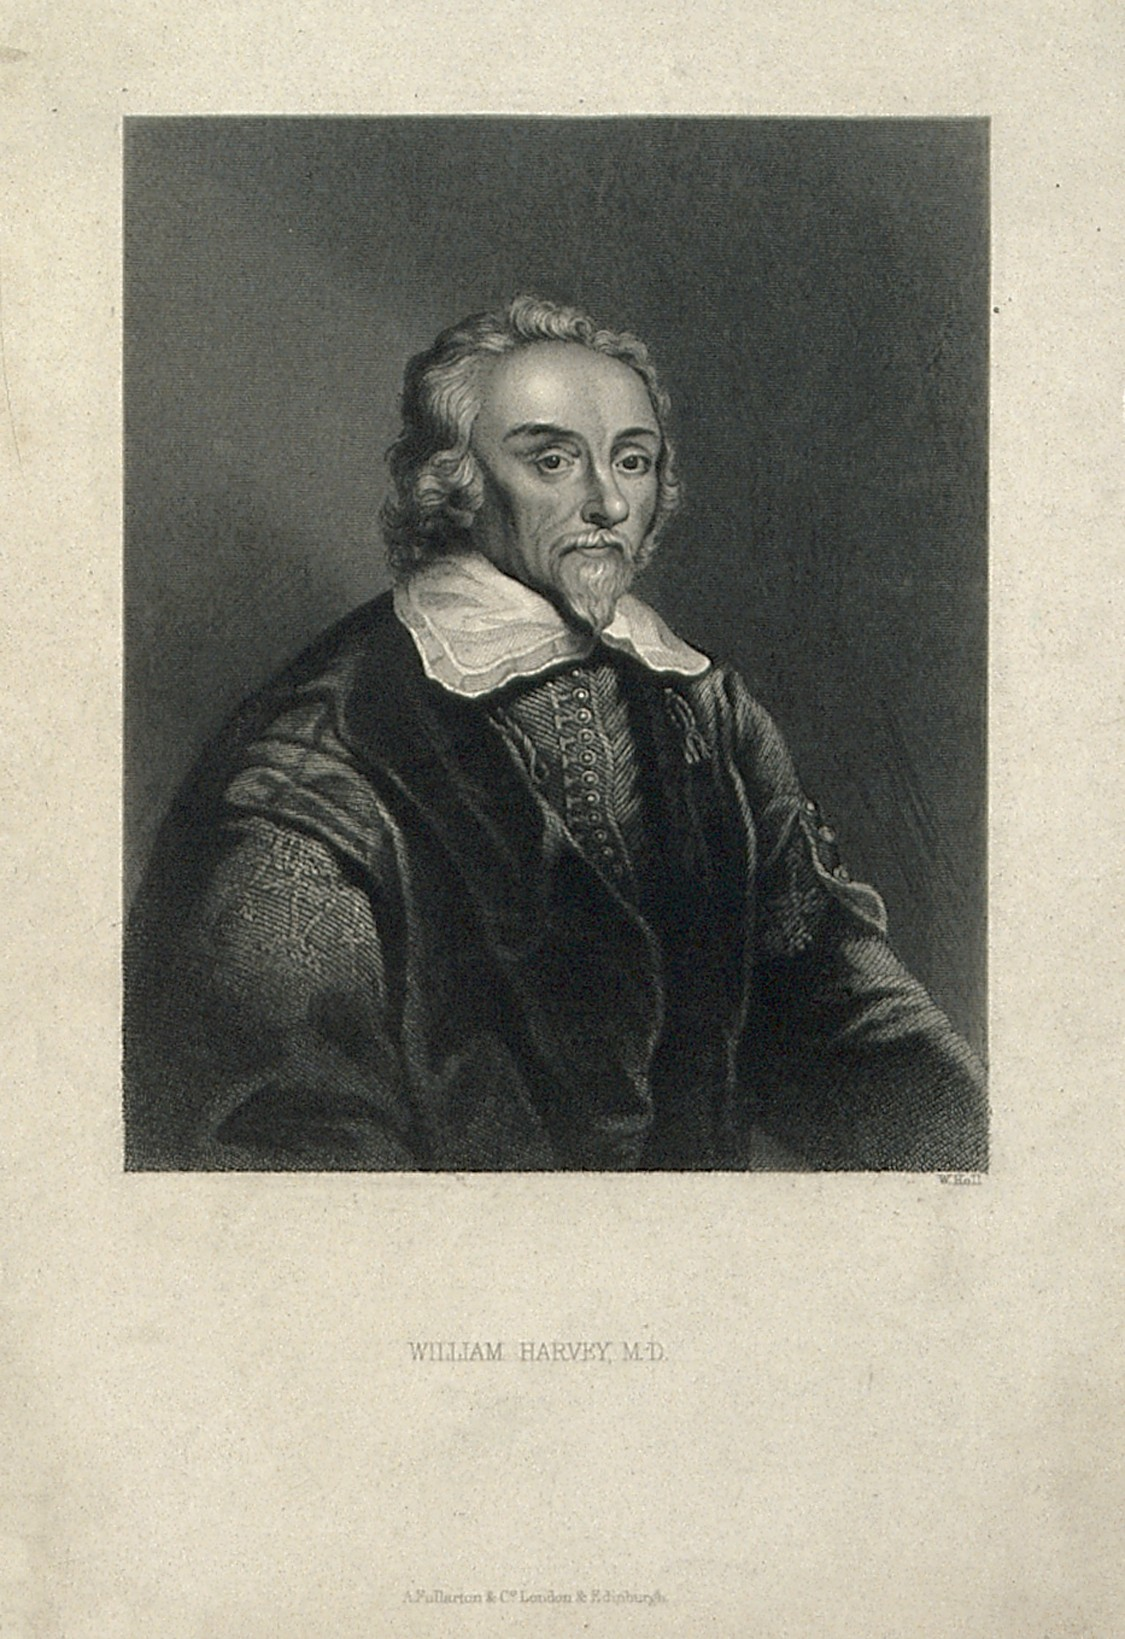
\includegraphics[width=0.3\linewidth]{images/book4/harvey.jpg}\hspace{0.05\linewidth}
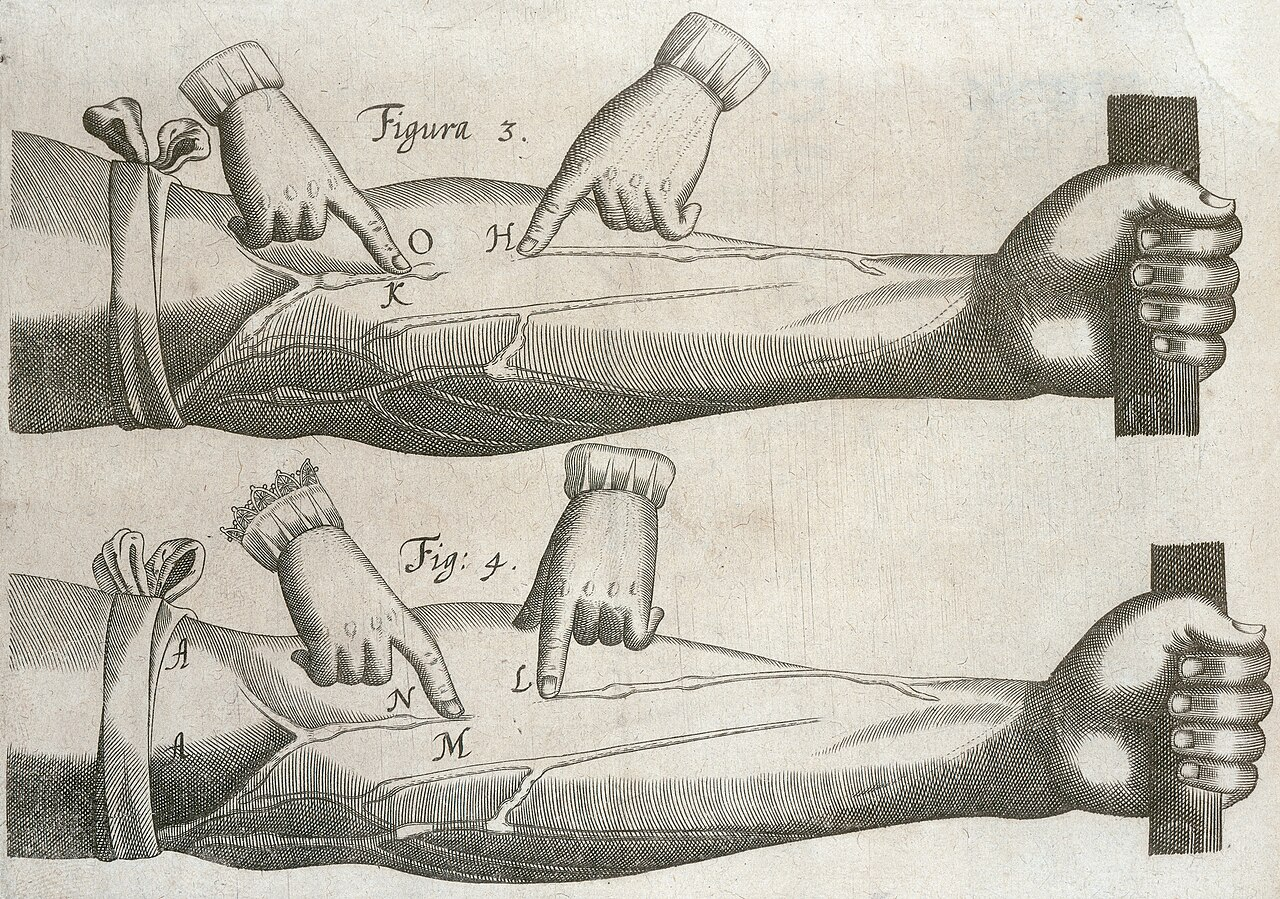
\includegraphics[width=0.42\linewidth]{images/book4/harvey-veins.jpg}

{\small William Harvey, en de plaat uit zijn boek van 1628: de \omterm{def:b2:blood-circulation:vessels}{aders} van een
afgebonden onderarm zwellen onder het koord op, en \omterm{def:b2:blood-circulation:blood}{bloed} dat naar de hand
wordt geduwd, stopt bij de kleppen.}
\end{omfigure}

\begin{omfigure}
\begin{tikzpicture}[every node/.style={font=\scriptsize}, >=stealth]
  % lungs and body
  \node[draw, rounded corners, fill=omDef!12, minimum width=3.4cm, minimum height=0.9cm] (lung) at (0,3) {longen: haarvaten van de longen};
  \node[draw, rounded corners, fill=omExo!25, minimum width=3.4cm, minimum height=0.9cm] (body) at (0,-3) {lichaam: haarvaten van het lichaam};
  % heart chambers
  \node[draw, fill=omDef!25, minimum width=1.3cm, minimum height=0.7cm] (ra) at (-1.6,0.6) {rechteratrium};
  \node[draw, fill=omDef!35, minimum width=1.3cm, minimum height=0.9cm] (rv) at (-1.6,-0.5) {rechterventrikel};
  \node[draw, fill=omThm!20, minimum width=1.3cm, minimum height=0.7cm] (la) at (1.6,0.6) {linkeratrium};
  \node[draw, fill=omThm!35, minimum width=1.3cm, minimum height=0.9cm] (lv) at (1.6,-0.5) {linkerventrikel};
  \draw[->, thick] (ra) -- (rv); \draw[->, thick] (la) -- (lv);
  % pulmonary circuit
  \draw[->, very thick, omDef] (rv.west) -- ++(-1.4,0) |- (lung.west) node[pos=0.25, left, align=right] {longslagader\\\qty{25}{mmHg}};
  \draw[->, very thick, omThm] (lung.east) -| (la.east) node[pos=0.75, right, align=left] {longaders\\zuurstofrijk};
  % systemic circuit
  \draw[->, very thick, omThm] (lv.east) -- ++(1.4,0) |- (body.east) node[pos=0.25, right, align=left] {aorta\\\qty{120}{mmHg}};
  \draw[->, very thick, omDef] (body.west) -| (ra.west);
  \node[omDef, anchor=east, align=right] at (-2.45,-1.6) {holle aders\\\qty{5}{mmHg}};
  \node[anchor=north, align=center] at (0,-3.7) {dezelfde stroom door beide kringlopen:\\\qty{5}{L/min} in rust};
\end{tikzpicture}

{\small De \omterm{def:b2:blood-circulation:circuits}{dubbele bloedsomloop}. Het rechterhart stuurt het \omterm{def:b2:blood-circulation:blood}{bloed} onder lage
druk door de longen; het linkerhart stuurt het onder hoge druk rond het
lichaam; de twee pompen, in serie, verplaatsen hetzelfde volume per minuut.}
\end{omfigure}

\section{Vaten en de fysica van de stroming}

\begin{definition}[De vaatboom]\label{def:b2:blood-circulation:vessels}
\index{slagader}\index{arteriole}\index{haarvat}\index{ader}
Het \omterm{def:b2:blood-circulation:blood}{bloed} verlaat het hart via \emph{slagaders}: dikwandige buizen met
elastische lagen die bij elke slag uitrekken en tussen de slagen
terugveren, waardoor de pulsen tot een gelijkmatiger stroom worden
afgevlakt (de aorta is \qty{2.5}{cm} breed). Ze vertakken zich tot
\emph{arteriolen}, vaten van een tiende millimeter of minder waarvan de
wand vooral uit glad spierweefsel bestaat: door samen te trekken of te
ontspannen verandert een arteriole haar straal en daarmee, sterk, haar
weerstand --- arteriolen zijn de kranen van de bloedsomloop en de plaats
van het grootste deel van de drukval. Ze monden uit in \emph{haarvaten}:
buisjes van één endotheelcel rond een lumen van \qtyrange{5}{10}{\micro m},
ongeveer \qty{1}{mm} lang, zo'n veertig miljard in getal met een totaal
oppervlak van bijna \qty{600}{m^2}, door de wand waarvan alle uitwisseling
plaatsvindt. Haarvaten monden uit in venulen en \emph{aders}: dunwandig,
rekbaar, met twee derde van het \omterm{def:b2:blood-circulation:blood}{bloed} onder lage druk, en met kleppen die de
stroming naar het hart gericht houden terwijl spieren ze samendrukken. Elk
vat is bekleed met één laag \emph{endotheel}, dat geen passieve bekleding is
maar een klier --- het geeft stikstofmonoxide af om de arteriole te
ontspannen, en signalen die witte bloedcellen rekruteren --- en een filter.
\end{definition}

\begin{omfigure}
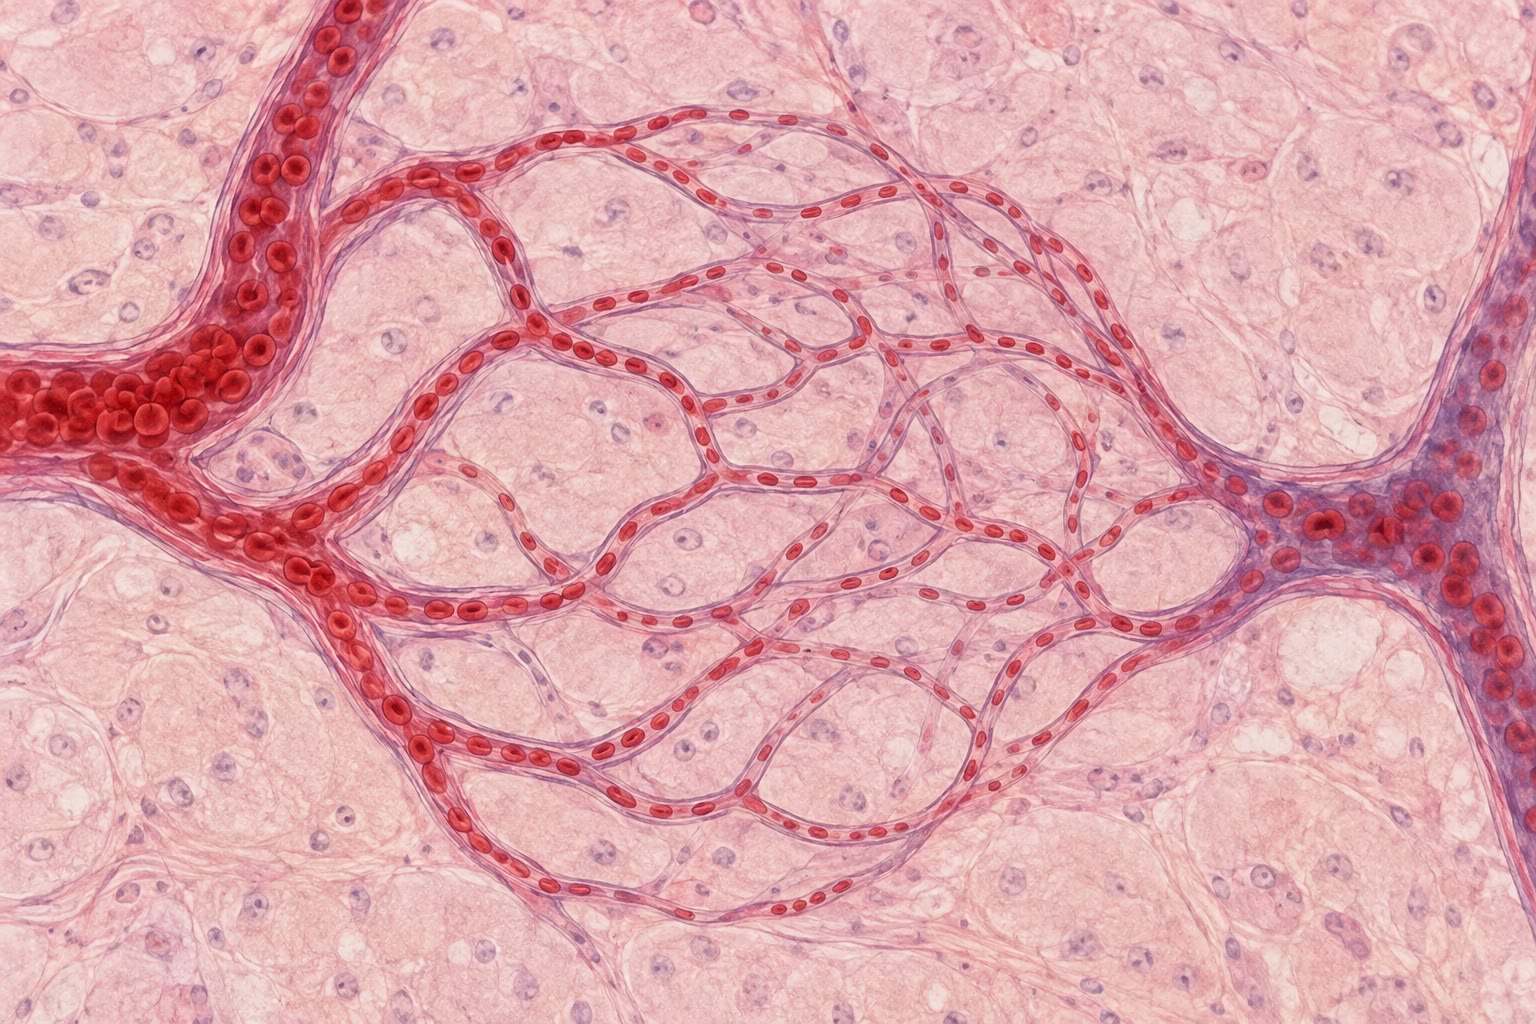
\includegraphics[width=0.55\linewidth]{images/book4/ai/b4-16-capillary-bed.jpg}

{\small Een haarvatennet: een \omterm{def:b2:blood-circulation:vessels}{arteriole} die een netwerk van \omterm{def:b2:blood-circulation:vessels}{haarvaten} voedt,
waarin rode bloedcellen achter elkaar reizen, en die samenkomen in een venule.}
\end{omfigure}

\begin{theorem}[De wet van Poiseuille en de vaatweerstand]\label{thm:b2:blood-circulation:poiseuille}
\index{wet van Poiseuille}\index{vaatweerstand}
De stationaire stroom $Q$ van een vloeistof met viscositeit $\eta$ door een
buis met straal $r$ en lengte $L$ onder een drukverschil $\Delta P$
is
\[
Q = \frac{\pi r^{4}}{8\eta L}\,\Delta P, \qquad \text{zodat}\qquad
R \equiv \frac{\Delta P}{Q} = \frac{8\eta L}{\pi r^{4}} .
\]
De weerstand daalt met de \emph{vierde macht} van de straal: een \omterm{def:b2:blood-circulation:vessels}{arteriole}
die haar straal met \qty{20}{\%} verkleint, vermenigvuldigt haar weerstand
met $1/0.8^{4} = 2.4$, en een die hem halveert met 16. Daarom kunnen een
paar millimeter arteriolaire spier het \omterm{def:b2:blood-circulation:blood}{bloed} van het hele lichaam omleiden
--- naar de darm na een maaltijd, naar de spieren bij inspanning, naar de
huid bij hitte --- en daarom daalt de druk van \qty{95}{mmHg} in de kleine
\omterm{def:b2:blood-circulation:vessels}{slagaders} tot \qty{35}{mmHg} bij de ingang van de \omterm{def:b2:blood-circulation:vessels}{haarvaten}, bijna volledig
over de \omterm{def:b2:blood-circulation:vessels}{arteriolen}, terwijl de daling langs de aorta een fractie van een
millimeter kwik bedraagt.
\end{theorem}
\begin{proof}
Bij stationaire laminaire stroming beweegt de vloeistof in concentrische
schillen; de viskeuze kracht tussen de schillen houdt de druk in evenwicht.
Voor de cilinder met straal $s < r$ is de drukkracht $\pi s^{2}\Delta P$
gelijk aan de viskeuze wrijving op zijn oppervlak $2\pi s L\,\eta\,(-\mathrm{d}v/
\mathrm{d}s)$, dus $\mathrm{d}v/\mathrm{d}s = -s\Delta P/(2\eta L)$
en, met $v(r) = 0$, $v(s) = (\Delta P/4\eta L)(r^{2} - s^{2})$ --- een
parabolisch profiel. Integreren van de snelheid over de doorsnede geeft
$Q = \int_{0}^{r} v\,2\pi s\,\mathrm{d}s = (\pi\Delta P/2\eta L)
\int_{0}^{r}(r^{2}s - s^{3})\,\mathrm{d}s = \pi r^{4}\Delta P/8\eta
L$. (\omterm{def:b2:blood-circulation:blood}{Bloed} is niet helemaal een eenvoudige vloeistof en \omterm{def:b2:blood-circulation:vessels}{slagaders} zijn niet
star, maar de vierdemachtswet geldt goed genoeg om een lichaam te laten
werken.)
\end{proof}

\begin{theorem}[Continuïteit: waar het bloed vertraagt]\label{thm:b2:blood-circulation:continuity}
\index{continuïteitsvergelijking}
Hetzelfde volume per seconde passeert elk niveau van de boom, zodat de
gemiddelde snelheid op een niveau $v = Q/A$ is, met $A$ de \emph{totale}
doorsnede van alle vaten op dat niveau. De aorta
(\qty{3}{cm^2}) voert \qty{5}{L/min} met \qty{28}{cm/s}; de \omterm{def:b2:blood-circulation:vessels}{haarvaten}, met
een totale doorsnede van bijna \qty{3000}{cm^2}, voeren het met
\qty{0.03}{cm/s}, zodat een \omterm{def:b2:blood-circulation:blood}{rode bloedcel} ongeveer drie seconden nodig heeft om
een \omterm{def:b2:blood-circulation:vessels}{haarvat} te doorkruisen --- tijd genoeg om haar zuurstof te laten
wegdiffunderen (\cref{ch:b2:unicellular-diversity}: een micrometer in een
milliseconde). De \omterm{def:b2:blood-circulation:vessels}{aders}, met een kleinere totale doorsnede dan de
\omterm{def:b2:blood-circulation:vessels}{haarvaten}, versnellen het \omterm{def:b2:blood-circulation:blood}{bloed} weer tot \qty{10}{cm/s} in de holle \omterm{def:b2:blood-circulation:vessels}{aders}.
De boom is zo gebouwd dat het \omterm{def:b2:blood-circulation:blood}{bloed} traag is precies waar het moet
uitwisselen en overal elders snel.
\end{theorem}
\begin{proof}
Behoud van volume: wat per seconde een niveau binnenkomt, verlaat het ook,
zodat $Q = A\,v$ op elk niveau hetzelfde is. $\qty{5}{L/min} =
\qty{83}{cm^3/s}$; $83/3 = \qty{28}{cm/s}$; $83/3000 =
\qty{0.028}{cm/s}$.
\end{proof}

\begin{omfigure}
\begin{tikzpicture}
\begin{axis}[
  width=0.9\linewidth, height=6.4cm,
  axis x line=bottom, axis y line=left,
  xmin=0, xmax=7, ymin=0, ymax=130,
  xtick={0.5,1.5,2.5,3.5,4.5,5.5,6.5},
  xticklabels={aorta, slagaders, arteriolen, haarvaten, venulen, aders, holle aders},
  x tick label style={font=\scriptsize, rotate=30, anchor=north east},
  ylabel={druk (\unit{mmHg})}, ylabel style={font=\small, omThm},
  tick label style={font=\small}, ytick={0,40,80,120},
  legend style={font=\scriptsize, at={(0.97,0.95)}, anchor=north east, draw=none},
  clip=false,
]
\addplot[very thick, omThm] coordinates {(0,120) (0.5,118) (1,110) (1.5,100) (2,95) (2.5,60) (3,35) (3.5,25) (4,15) (4.5,12) (5,8) (5.5,5) (6,4) (6.5,3) (7,2)};
\addlegendentry{gemiddelde druk}
\addplot[very thick, omThm, dashed] coordinates {(0,120) (0.5,120) (1,125) (1.5,120) (2,100)};
\addplot[very thick, omThm, dashed] coordinates {(0,80) (0.5,80) (1,80) (1.5,82) (2,88)};
\addlegendentry{systolisch en diastolisch}
\end{axis}
\begin{axis}[
  width=0.9\linewidth, height=6.4cm,
  axis x line=none, axis y line=right,
  xmin=0, xmax=7, ymin=0, ymax=32,
  ylabel={snelheid (\unit{cm/s})}, ylabel style={font=\small, omDef},
  tick label style={font=\small}, ytick={0,10,20,30},
  legend style={font=\scriptsize, at={(0.97,0.72)}, anchor=north east, draw=none},
  clip=false,
]
\addplot[very thick, omDef] coordinates {(0,28) (0.5,26) (1,18) (1.5,10) (2,5) (2.5,1.5) (3,0.3) (3.5,0.03) (4,0.3) (4.5,1.5) (5,4) (5.5,7) (6,9) (6.5,10) (7,10)};
\addlegendentry{gemiddelde snelheid}
\end{axis}
\end{tikzpicture}

{\small Druk (rood) en gemiddelde snelheid (blauw) langs de \omterm{def:b2:blood-circulation:circuits}{grote
bloedsomloop}. De pols wordt in de \omterm{def:b2:blood-circulation:vessels}{slagaders} afgevlakt, de druk daalt vooral
over de \omterm{def:b2:blood-circulation:vessels}{arteriolen}, en het \omterm{def:b2:blood-circulation:blood}{bloed} is het traagst in de \omterm{def:b2:blood-circulation:vessels}{haarvaten}, waar de
totale doorsnede duizend keer die van de aorta is.}
\end{omfigure}

\begin{theorem}[De elastische slagader als reservoir]\label{thm:b2:blood-circulation:windkessel}
\index{Windkessel}\index{compliantie!arteriële}\index{polsdruk}
Het hart pompt met stoten; de weefsels ontvangen een bijna gelijkmatige
stroom. De grote \omterm{def:b2:blood-circulation:vessels}{slagaders} zorgen voor de afvlakking: ze rekken uit tijdens
de uitstoting, slaan een deel van het slagvolume op, en veren tijdens de
diastole terug, waardoor ze het verder drijven. Als de \omterm{def:b2:blood-circulation:vessels}{slagaders} een
\emph{compliantie}
$C$ hebben (opgeslagen volume per eenheid druk) en de \omterm{def:b2:blood-circulation:vessels}{arteriolen} een
weerstand $R$, dan daalt de druk tijdens de diastole, met de aortaklep
gesloten, als
\[
P(t) = P_{s}\,e^{-t/RC},
\]
zodat de diastolische druk na een diastole van duur $t_d$ gelijk is
aan $P_s e^{-t_d/RC}$: met $R = \qty{1}{mmHg.s/mL}$, $C =
\qty{2}{mL/mmHg}$ en $t_d = \qty{0.8}{s}$ daalt een systolische druk van
\qty{120}{mmHg} tot \qty{80}{mmHg}. Een stijvere aorta (kleinere
$C$, zoals op hoge leeftijd) laat de druk tussen de slagen verder dalen
en tijdens de uitstoting hoger stijgen: de \emph{\omterm{thm:b2:blood-circulation:windkessel}{polsdruk}} wordt groter,
en het hart werkt tegen een hogere piek in.
\end{theorem}
\begin{proof}
Tijdens de diastole komt er geen \omterm{def:b2:blood-circulation:blood}{bloed} in de \omterm{def:b2:blood-circulation:vessels}{slagaders} en verlaat het ze via
de \omterm{def:b2:blood-circulation:vessels}{arteriolen} met $Q = P/R$; het arteriële volume daalt met
$\mathrm{d}V/\mathrm{d}t = -P/R$, en omdat $\mathrm{d}V = C\,
\mathrm{d}P$, geldt $C\,\mathrm{d}P/\mathrm{d}t = -P/R$, met als oplossing
de exponentiële functie met tijdconstante $RC$. Met $RC = \qty{2}{s}$:
$120\,e^{-0.4} = \qty{80}{mmHg}$.
\end{proof}

\section{Uitwisseling in de haarvaten}

\begin{proposition}[Twee soorten uitwisseling]\label{prop:b2:blood-circulation:exchange}
\index{capillaire uitwisseling}\index{krachten van Starling}\index{oedeem}\index{lymfe}
Door de haarvatwand bewegen opgeloste stoffen door \emph{diffusie} ---
gassen en lipiden door de cellen, water en kleine opgeloste stoffen door de
spleten ertussen, over het enorme oppervlak en de korte afstand die de flux
ruim voldoende maken (de wet van Fick, zoals voor de \omterm{def:b2:mammal-reproduction:placenta}{placenta} van
\cref{ch:b2:mammal-reproduction}) --- en beweegt water door
\emph{massastroming}, gedreven door het evenwicht tussen twee drukken. De
hydrostatische druk in het \omterm{def:b2:blood-circulation:vessels}{haarvat}, $P_c$, duwt vloeistof naar buiten; de
\omterm{thm:b2:blood-circulation:oncotic}{oncotische druk} van de plasma-eiwitten, $\pi_c$, trekt haar naar binnen
(\emph{\omterm{prop:b2:blood-circulation:exchange}{krachten van Starling}}). Aan het arteriële uiteinde overtreft
$P_c \approx
\qty{35}{mmHg}$ de $\pi_c \approx \qty{25}{mmHg}$ en filtreert vloeistof
naar buiten; aan het veneuze uiteinde is $P_c \approx \qty{15}{mmHg}$ en
wordt vloeistof teruggeresorbeerd; over het hele lichaam filtreert er
ongeveer \qty{20}{L} per dag naar buiten en keert er \qty{17}{L} terug, en het
saldo van \qty{3}{L}, met de eiwitten die zijn weggelekt, wordt door de
\emph{lymfevaten} verzameld en ter hoogte van de hals aan de \omterm{def:b2:blood-circulation:vessels}{aders}
teruggegeven. \emph{Oedeem} --- zwelling door vocht in de weefsels ---
volgt telkens wanneer het evenwicht doorslaat: een hoge veneuze druk
(hartfalen), een laag plasma-eiwit (ondervoeding, lever- of nierziekte),
lekkende \omterm{def:b2:blood-circulation:vessels}{haarvaten} (ontsteking), of verstopte lymfevaten.
\end{proposition}

\begin{omfigure}
\begin{tikzpicture}[every node/.style={font=\scriptsize}, >=stealth]
  % capillary
  \draw[thick, fill=omThm!10] (0,0) rectangle (9,1.2);
  \node[left] at (-0.1,0.6) {arteriole};
  \node[right] at (9.1,0.6) {venule};
  \draw[->, very thick, omThm] (0.3,0.6) -- (8.7,0.6);
  % pressures
  \node[above, align=center] at (1.5,1.3) {arterieel uiteinde\\$P_c = 35$, $\pi_c = 25$};
  \node[above, align=center] at (7.5,1.3) {veneus uiteinde\\$P_c = 15$, $\pi_c = 25$};
  \foreach \x in {0.8,1.5,2.2} \draw[->, thick, omDef] (\x,0) -- (\x,-0.7);
  \node[below, align=center, omDef] at (1.5,-0.75) {netto $+10$ mmHg:\\filtratie};
  \foreach \x in {6.8,7.5,8.2} \draw[->, thick, omDef] (\x,-0.7) -- (\x,0);
  \node[below, align=center, omDef] at (7.5,-0.75) {netto $-10$ mmHg:\\resorptie};
  \draw[->, thick, omExo!70!black] (4.5,-0.4) -- (4.5,-1.6) node[below, align=center] {overschot naar de lymfe:\\\qty{3}{L} per dag};
  \node[align=center] at (4.5,-0.15) {interstitieel vocht};
\end{tikzpicture}

{\small \omterm{prop:b2:blood-circulation:exchange}{Krachten van Starling} langs een \omterm{def:b2:blood-circulation:vessels}{haarvat}. De hydrostatische druk duwt
vloeistof naar buiten en de \omterm{thm:b2:blood-circulation:oncotic}{oncotische druk} van de plasma-eiwitten trekt ze
terug; de filtratie aan het arteriële uiteinde overtreft de resorptie aan
het veneuze uiteinde, en de lymfe voert het verschil terug.}
\end{omfigure}

\begin{theorem}[Oncotische druk]\label{thm:b2:blood-circulation:oncotic}
\index{oncotische druk}\index{albumine}
Een oplossing van $c$ mol per liter van een opgeloste stof die een membraan
niet kan passeren, oefent over dat membraan een osmotische druk
$\pi = cRT$ uit (van 't
Hoff). Plasma-albumine, \qty{40}{g/L} van een eiwit met molaire massa
\qty{66}{kg/mol}, is $c = \qty{0.6}{mmol/L}$ en geeft $\pi =
0.6\times 8.314\times 310 = \qty{1.55}{kPa} \approx \qty{12}{mmHg}$;
de andere eiwitten en de extra ionen die de negatieve lading van albumine
vasthoudt, brengen het totaal op ongeveer \qty{25}{mmHg}. Het
natriumchloride van het \omterm{def:b2:blood-circulation:blood}{plasma}, met \qty{150}{mmol/L}, zou
\qty{5800}{mmHg} uitoefenen --- maar het passeert de haarvatwand vrij en
oefent er geen druk over uit. Voor het \omterm{def:b2:blood-circulation:vessels}{haarvat} telt het eiwit: halveer de
albumine, zoals bij een nierziekte die haar in de urine verliest, en de
resorberende trek halveert, vocht hoopt zich in de weefsels op, en de
patiënt zwelt op.
\end{theorem}
\begin{proof}
$\qty{40}{g/L}/\qty{66000}{g/mol} = \qty{6.1e-4}{mol/L} =
\qty{0.61}{mol/m^3}$; $\pi = cRT = 0.61\times 8.314\times 310 =
\qty{1570}{Pa}$; $\qty{1}{mmHg} = \qty{133}{Pa}$, dus \qty{11.8}{mmHg}.
De wet van van 't Hoff zelf is de limiet voor verdunde oplossingen die in
het deel van jaar 1 is afgeleid.
\end{proof}

\begin{example}[De bloedsomloop als vervoerssysteem]\label{ex:b2:blood-circulation:transport}
Vijf liter per minuut door \qty{600}{m^2} haarvatwand is een bezorgdienst
zonder weerga. Hij brengt elke cel zuurstof tot op enkele celdiameters
(geen enkele cel van het lichaam ligt verder dan \qty{20}{\micro m} van een
\omterm{def:b2:blood-circulation:vessels}{haarvat}), voert haar $\mathrm{CO_2}$, lactaat en ureum af, brengt de glucose
van de lever naar de hersenen en de vetzuren van de vetvoorraden naar de
spieren, verdeelt de hormonen van \cref{ch:b2:cell-signalling} in een minuut
van één klier naar elke receptor in het lichaam, vervoert de warmte van de
kern naar de huid en terug, en brengt de witte bloedcellen binnen enkele
uren naar een wond. Het is ook de kwetsbaarheid: een stolsel, een bloeding
of een falende pomp legt alles tegelijk stil, en de hersenen, die geen
brandstof opslaan, vallen binnen seconden uit. De rest van dit deel van het
boek gaat over de pomp (\cref{ch:b2:heart}) en over hoe de druk wordt
geregeld, zodat de dienst doorgaat bij het opstaan, bij het hardlopen en bij
een bloeding (\cref{ch:b2:blood-pressure}).
\end{example}

\section{Opgaven}

\begin{exercise}[$\star$]\label{exo:b2:blood-circulation:1}
Geef de volumesamenstelling van \omterm{def:b2:blood-circulation:blood}{bloed} en het aantal, de grootte en de
functie van elk cellulair bestanddeel.
\end{exercise}

\begin{exercise}[$\star$]\label{exo:b2:blood-circulation:2}
Teken de bloedsomloop van een vis en van een zoogdier, geef de drukken aan,
en zeg wat de dubbele kringloop oplevert.
\end{exercise}

\begin{exercise}[$\star$]\label{exo:b2:blood-circulation:3}
Geef voor elk vaattype --- \omterm{def:b2:blood-circulation:vessels}{slagader}, \omterm{def:b2:blood-circulation:vessels}{arteriole}, \omterm{def:b2:blood-circulation:vessels}{haarvat}, \omterm{def:b2:blood-circulation:vessels}{ader} --- de bouw van
de wand en de functie die hij dient.
\end{exercise}

\begin{exercise}[$\star$]\label{exo:b2:blood-circulation:4}
Reconstrueer het argument van Harvey vanuit de hoeveelheid, met moderne
getallen: \qty{70}{mL} per slag, \num{72} slagen per minuut, \qty{5}{L} \omterm{def:b2:blood-circulation:blood}{bloed}.
\end{exercise}

\begin{exercise}[$\star\star$]\label{exo:b2:blood-circulation:5}
Bereken met de \omterm{thm:b2:blood-circulation:poiseuille}{wet van Poiseuille} de drukval langs de aorta (straal
\qty{1.25}{cm}, lengte \qty{40}{cm}, $\eta = \qty{3e-3}{Pa.s}$) bij
\qty{5}{L/min}, in pascal en in mmHg. Becommentarieer.
\end{exercise}

\begin{exercise}[$\star\star$]\label{exo:b2:blood-circulation:6}
Een \omterm{def:b2:blood-circulation:vessels}{arteriole} met straal \qty{15}{\micro m} vernauwt tot
\qty{12}{\micro m} en verwijdt daarna tot \qty{20}{\micro m}. Met welke
factor verandert haar weerstand in elk geval, en haar stroom bij constante
druk?
\end{exercise}

\begin{exercise}[$\star\star$]\label{exo:b2:blood-circulation:7}
De aorta heeft een doorsnede van \qty{3}{cm^2} en de \omterm{def:b2:blood-circulation:vessels}{haarvaten} samen
\qty{3000}{cm^2}; de stroom is \qty{5}{L/min}. Bereken de gemiddelde snelheid
in elk, en de tijd die een \omterm{def:b2:blood-circulation:blood}{rode bloedcel} in een \omterm{def:b2:blood-circulation:vessels}{haarvat} van \qty{1}{mm}
doorbrengt. Bij inspanning stijgt het debiet tot \qty{25}{L/min} en gaan de
\omterm{def:b2:blood-circulation:vessels}{haarvaten} van de spieren open: wat gebeurt er met de doorlooptijd?
\end{exercise}

\begin{exercise}[$\star\star$]\label{exo:b2:blood-circulation:8}
Bereken met $P_c = 35$ en \qty{15}{mmHg} aan de twee uiteinden,
$\pi_c =
\qty{25}{mmHg}$ en verwaarloosbare interstitiële drukken de netto
filtratiedruk aan elk uiteinde. Wat gebeurt er als de veneuze druk zo
stijgt dat $P_c$ aan het veneuze uiteinde \qty{28}{mmHg} is?
\end{exercise}

\begin{exercise}[$\star\star$]\label{exo:b2:blood-circulation:9}
Bereken de \omterm{thm:b2:blood-circulation:oncotic}{oncotische druk} van \qty{40}{g/L} albumine
(\qty{66}{kg/mol}) bij \qty{37}{\celsius}, en die van \qty{20}{g/L}. Waarom
draagt het natrium van het \omterm{def:b2:blood-circulation:blood}{plasma}, met \qty{150}{mmol/L}, niets bij aan het
evenwicht van Starling?
\end{exercise}

\begin{exercise}[$\star\star\star$]\label{exo:b2:blood-circulation:10}
Bereken met $R = \qty{1}{mmHg.s/mL}$ en $C = \qty{2}{mL/mmHg}$ de
diastolische druk na \qty{0.8}{s}, uitgaande van een systolische druk van
\qty{120}{mmHg}. Bereken het opnieuw voor een aorta die half zo rekbaar is.
Leg uit waarom de \omterm{thm:b2:blood-circulation:windkessel}{polsdruk} van ouderen groot is, en wat dat het hart kost.
\end{exercise}

\begin{exercise}[$\star\star\star$]\label{exo:b2:blood-circulation:11}
De systemische weerstand is $R = (P_{\text{art}} - P_{\text{ven}})/Q$.
Bereken hem in rust ($95 - 5$ mmHg, \qty{5}{L/min}) en bij inspanning
($110 - 5$, \qty{25}{L/min}). Met welke factor moet de gemiddelde straal van
de \omterm{def:b2:blood-circulation:vessels}{arteriolen} zijn veranderd, als de \omterm{def:b2:blood-circulation:vessels}{arteriolen} de hele weerstand dragen?
\end{exercise}

\begin{exercise}[$\star\star\star$]\label{exo:b2:blood-circulation:12}
``De bloedsomloop is zo gebouwd dat het \omterm{def:b2:blood-circulation:blood}{bloed} traag is waar het moet
uitwisselen en overal elders snel.'' Bespreek dit aan de hand van de
\omterm{thm:b2:blood-circulation:continuity}{continuïteitsvergelijking}, de \omterm{thm:b2:blood-circulation:poiseuille}{wet van Poiseuille} en de meetkunde van de
boom, en zeg waarom een \omterm{def:b2:blood-circulation:circuits}{open bloedsomloop} dat niet kan.
\end{exercise}

\section{Vraagstuk: de bloedsomloop in getallen}

\begin{problem}[{Weekendvraagstuk --- de rekensom van Harvey overgedaan, de
drukken en snelheden van de vaatboom berekend met Poiseuille en de
continuïteit, de dagelijkse filtratie van de haarvaten sluitend gemaakt, en
de afvlakking door de aorta gemodelleerd, met als besluit het
hartminuutvolume, de drukval over de arteriolen, het filtraat van een dag en
de diastolische druk}]
\label{pb:b2:blood-circulation:1}
Gegevens: slagvolume \qty{70}{mL}, hartfrequentie \qty{72}{min^{-1}},
bloedvolume \qty{5}{L}, $\eta = \qty{3e-3}{Pa.s}$, $\qty{1}{mmHg} =
\qty{133}{Pa}$. Aorta: straal \qty{1.25}{cm}, lengte \qty{40}{cm}.
\omterm{def:b2:blood-circulation:vessels}{Arteriolen}: $3\times 10^{6}$ parallel geschakeld, elk met straal
\qty{15}{\micro m} en lengte \qty{1}{mm}. \omterm{def:b2:blood-circulation:vessels}{Haarvaten}: $4\times
10^{10}$, straal \qty{3}{\micro m}, lengte \qty{1}{mm}, waarvan in rust een
kwart open. Starling: $P_c$ van 35 tot \qty{15}{mmHg} langs een \omterm{def:b2:blood-circulation:vessels}{haarvat},
$\pi_c = \qty{25}{mmHg}$. Windkessel: $C =
\qty{2}{mL/mmHg}$, diastole \qty{0.8}{s}.

\medskip
\noindent\textbf{Deel I --- De rekensom van Harvey.}
\begin{enumerate}
  \item Bereken het hartminuutvolume in liter per minuut en per dag.
  \item Hoe vaak per dag circuleert het bloedvolume?
  \item De schatting van Harvey was 2~oncen (\qty{57}{g}) per slag, waarvan
        volgens hem minstens een kwart werd uitgestoten, bij 72 slagen per
        minuut. Welke massa \omterm{def:b2:blood-circulation:blood}{bloed} gaf dat per uur, en hoe verhield die zich
        tot het gewicht van een man?
  \item Waarom was dit een argument voor een kringloop en niet voor
        voortdurende aanmaak en verbruik?
  \item Beschrijf het afbindexperiment en wat de kleppen aantoonden.
  \item Wat kon Harvey niet zien, en wie zag het wel?
\end{enumerate}

\medskip
\noindent\textbf{Deel II --- De boom.}
\begin{enumerate}[resume]
  \item Bereken de gemiddelde snelheid in de aorta.
  \item Bereken met de \omterm{thm:b2:blood-circulation:poiseuille}{wet van Poiseuille} de drukval langs de aorta, in
        mmHg.
  \item Bereken de weerstand van één \omterm{def:b2:blood-circulation:vessels}{arteriole} en van de $3\times
        10^{6}$ parallel geschakelde.
  \item Bereken de drukval over de \omterm{def:b2:blood-circulation:vessels}{arteriolen} bij het rustdebiet, in mmHg.
  \item Bereken de totale doorsnede van de open \omterm{def:b2:blood-circulation:vessels}{haarvaten} en de gemiddelde
        snelheid daarin; daarna de doorlooptijd door één \omterm{def:b2:blood-circulation:vessels}{haarvat}.
  \item De \omterm{def:b2:blood-circulation:vessels}{arteriolen} vernauwen zich zodat hun straal met \qty{10}{\%}
        afneemt. Bereken de drukval opnieuw. Wat moet het hart doen om
        hetzelfde debiet te behouden?
\end{enumerate}

\medskip
\noindent\textbf{Deel III --- De \omterm{def:b2:blood-circulation:vessels}{haarvaten}.}
\begin{enumerate}[resume]
  \item Bereken de netto filtratiedruk aan het arteriële uiteinde, aan het
        veneuze uiteinde en in het midden (neem aan dat $P_c$ lineair
        daalt).
  \item Verdeel het \omterm{def:b2:blood-circulation:vessels}{haarvat} in de filtrerende en de resorberende helft en
        schat de per dag gefiltreerde en geresorbeerde vloeistof over het
        hele lichaam, met als netto drukken, gemiddeld over elke helft,
        $+10$ en
        \qty{-8.5}{mmHg}, en met elke helft die \qty{2}{L} per dag per mmHg
        verplaatst.
  \item Leid de lymfestroom af.
  \item De plasma-albumine daalt tot \qty{20}{g/L}. Bereken $\pi_c$
        opnieuw (neem aan dat die met de albumine meeschaalt) en de netto
        drukken aan de twee uiteinden. Wat gebeurt er?
  \item De veneuze druk stijgt zodat $P_c$ loopt van 35 tot
        \qty{28}{mmHg}. Bereken opnieuw de gemiddelde netto druk en de
        dagelijkse balans. Waar gaat de vloeistof naartoe?
  \item Bereken het totale haarvatoppervlak (cilinders, allemaal) en de tijd
        die een molecuul nodig heeft om te diffunderen naar een cel op
        \qty{20}{\micro m} van een \omterm{def:b2:blood-circulation:vessels}{haarvat} ($D = \qty{1e-9}{m^2/s}$).
\end{enumerate}

\medskip
\noindent\textbf{Deel IV --- De aorta als reservoir.}
\begin{enumerate}[resume]
  \item Bereken de systemische weerstand uit een gemiddelde druk van
        \qty{93}{mmHg}, een veneuze druk van \qty{3}{mmHg} en het rustdebiet,
        in \unit{mmHg.s/mL}.
  \item Bereken de tijdconstante $RC$ en de diastolische druk na
        \qty{0.8}{s}, uitgaande van een systolische druk van \qty{120}{mmHg}.
  \item Bereken het opnieuw voor $C = \qty{1}{mL/mmHg}$. Wat is er met de
        \omterm{thm:b2:blood-circulation:windkessel}{polsdruk} gebeurd?
  \item De hartfrequentie stijgt tot \num{120} en de diastole verkort tot
        \qty{0.3}{s}. Bereken de diastolische druk.
  \item Hoeveel van de \qty{70}{mL} die worden uitgestoten, wordt tijdens de
        systole in de \omterm{def:b2:blood-circulation:vessels}{slagaders} opgeslagen als de druk met \qty{20}{mmHg}
        stijgt? Waar gaat de rest naartoe?
  \item Leg uit waarom de kransslagaders, die zich in de diastole vullen,
        afhangen van het terugveren van de aorta.
  \item Formuleer het resultaat: het hartminuutvolume, de drukval over de
        \omterm{def:b2:blood-circulation:vessels}{arteriolen}, het netto filtraat van een dag, en de diastolische druk
        voor $C = 2$ en $C = 1$.
\end{enumerate}
\end{problem}
